\subsection{Permanent}

\begin{frame}
    \tiny
    \frametitle{PERMANENT}

    La visualisation ci-dessous présente la répartition du CA par point de vente pour les achats de type \textbf{PERMANENT}.\par
    Pour rappel, le total de ce CA s’élève à \textbf{<< permanent['ca_total']|number(2) >>€} soit \textbf{<< part_ca_mode_permanent|number >>\% du CA total}.\par

    Le point de vente \textbf{<< permanent['magasin_plus_gros_ca']['nom'] >>} représente \textbf{<< permanent['magasin_plus_gros_ca']['part_ca']|number >>}\% du CA PERMANENT.\par

    \begin{figure}[h]
        \centering
        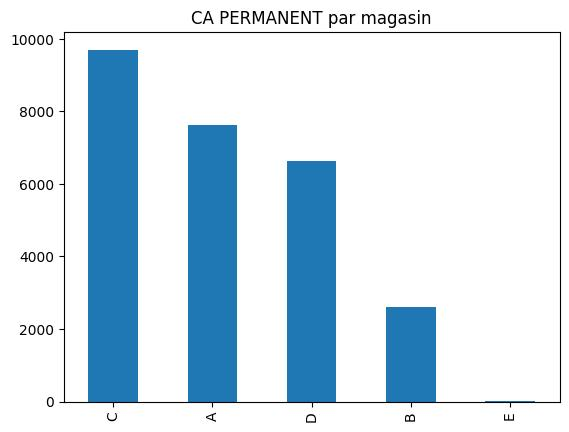
\includegraphics[height=3cm]{assets/__ca_permanent_par_magasin}
    \end{figure}
\end{frame}
